\documentclass{ximera}

%\usepackage{todonotes}

\newcommand{\todo}{}

\usepackage{esint} % for \oiint
\ifxake%%https://math.meta.stackexchange.com/questions/9973/how-do-you-render-a-closed-surface-double-integral
\renewcommand{\oiint}{{\large\bigcirc}\kern-1.56em\iint}
\fi


\graphicspath{
  {./}
  {ximeraTutorial/}
  {basicPhilosophy/}
  {functionsOfSeveralVariables/}
  {normalVectors/}
  {lagrangeMultipliers/}
  {vectorFields/}
  {greensTheorem/}
  {shapeOfThingsToCome/}
  {dotProducts/}
  {partialDerivativesAndTheGradientVector/}
  {../productAndQuotientRules/exercises/}
  {../normalVectors/exercisesParametricPlots/}
  {../continuityOfFunctionsOfSeveralVariables/exercises/}
  {../partialDerivativesAndTheGradientVector/exercises/}
  {../directionalDerivativeAndChainRule/exercises/}
  {../commonCoordinates/exercisesCylindricalCoordinates/}
  {../commonCoordinates/exercisesSphericalCoordinates/}
  {../greensTheorem/exercisesCurlAndLineIntegrals/}
  {../greensTheorem/exercisesDivergenceAndLineIntegrals/}
  {../shapeOfThingsToCome/exercisesDivergenceTheorem/}
  {../greensTheorem/}
  {../shapeOfThingsToCome/}
  {../separableDifferentialEquations/exercises/}
  {vectorFields/}
}

\newcommand{\mooculus}{\textsf{\textbf{MOOC}\textnormal{\textsf{ULUS}}}}

\usepackage{tkz-euclide}
\usepackage{tikz}
\usepackage{tikz-cd}
\usetikzlibrary{arrows}
\tikzset{>=stealth,commutative diagrams/.cd,
  arrow style=tikz,diagrams={>=stealth}} %% cool arrow head
\tikzset{shorten <>/.style={ shorten >=#1, shorten <=#1 } } %% allows shorter vectors

\usetikzlibrary{backgrounds} %% for boxes around graphs
\usetikzlibrary{shapes,positioning}  %% Clouds and stars
\usetikzlibrary{matrix} %% for matrix
\usepgfplotslibrary{polar} %% for polar plots
\usepgfplotslibrary{fillbetween} %% to shade area between curves in TikZ
%\usetkzobj{all}
\usepackage[makeroom]{cancel} %% for strike outs
%\usepackage{mathtools} %% for pretty underbrace % Breaks Ximera
%\usepackage{multicol}
\usepackage{pgffor} %% required for integral for loops



%% http://tex.stackexchange.com/questions/66490/drawing-a-tikz-arc-specifying-the-center
%% Draws beach ball
\tikzset{pics/carc/.style args={#1:#2:#3}{code={\draw[pic actions] (#1:#3) arc(#1:#2:#3);}}}



\usepackage{array}
\setlength{\extrarowheight}{+.1cm}
\newdimen\digitwidth
\settowidth\digitwidth{9}
\def\divrule#1#2{
\noalign{\moveright#1\digitwidth
\vbox{\hrule width#2\digitwidth}}}




% \newcommand{\RR}{\mathbb R}
% \newcommand{\R}{\mathbb R}
% \newcommand{\N}{\mathbb N}
% \newcommand{\Z}{\mathbb Z}

\newcommand{\sagemath}{\textsf{SageMath}}


%\renewcommand{\d}{\,d\!}
%\renewcommand{\d}{\mathop{}\!d}
%\newcommand{\dd}[2][]{\frac{\d #1}{\d #2}}
%\newcommand{\pp}[2][]{\frac{\partial #1}{\partial #2}}
% \renewcommand{\l}{\ell}
%\newcommand{\ddx}{\frac{d}{\d x}}

% \newcommand{\zeroOverZero}{\ensuremath{\boldsymbol{\tfrac{0}{0}}}}
%\newcommand{\inftyOverInfty}{\ensuremath{\boldsymbol{\tfrac{\infty}{\infty}}}}
%\newcommand{\zeroOverInfty}{\ensuremath{\boldsymbol{\tfrac{0}{\infty}}}}
%\newcommand{\zeroTimesInfty}{\ensuremath{\small\boldsymbol{0\cdot \infty}}}
%\newcommand{\inftyMinusInfty}{\ensuremath{\small\boldsymbol{\infty - \infty}}}
%\newcommand{\oneToInfty}{\ensuremath{\boldsymbol{1^\infty}}}
%\newcommand{\zeroToZero}{\ensuremath{\boldsymbol{0^0}}}
%\newcommand{\inftyToZero}{\ensuremath{\boldsymbol{\infty^0}}}



% \newcommand{\numOverZero}{\ensuremath{\boldsymbol{\tfrac{\#}{0}}}}
% \newcommand{\dfn}{\textbf}
% \newcommand{\unit}{\,\mathrm}
% \newcommand{\unit}{\mathop{}\!\mathrm}
% \newcommand{\eval}[1]{\bigg[ #1 \bigg]}
% \newcommand{\seq}[1]{\left( #1 \right)}
% \renewcommand{\epsilon}{\varepsilon}
% \renewcommand{\phi}{\varphi}


% \renewcommand{\iff}{\Leftrightarrow}

% \DeclareMathOperator{\arccot}{arccot}
% \DeclareMathOperator{\arcsec}{arcsec}
% \DeclareMathOperator{\arccsc}{arccsc}
% \DeclareMathOperator{\si}{Si}
% \DeclareMathOperator{\scal}{scal}
% \DeclareMathOperator{\sign}{sign}


%% \newcommand{\tightoverset}[2]{% for arrow vec
%%   \mathop{#2}\limits^{\vbox to -.5ex{\kern-0.75ex\hbox{$#1$}\vss}}}
% \newcommand{\arrowvec}[1]{{\overset{\rightharpoonup}{#1}}}
% \renewcommand{\vec}[1]{\arrowvec{\mathbf{#1}}}
% \renewcommand{\vec}[1]{{\overset{\boldsymbol{\rightharpoonup}}{\mathbf{#1}}}}

% \newcommand{\point}[1]{\left(#1\right)} %this allows \vector{ to be changed to \vector{ with a quick find and replace
% \newcommand{\pt}[1]{\mathbf{#1}} %this allows \vec{ to be changed to \vec{ with a quick find and replace
% \newcommand{\Lim}[2]{\lim_{\point{#1} \to \point{#2}}} %Bart, I changed this to point since I want to use it.  It runs through both of the exercise and exerciseE files in limits section, which is why it was in each document to start with.

% \DeclareMathOperator{\proj}{\mathbf{proj}}
% \newcommand{\veci}{{\boldsymbol{\hat{\imath}}}}
% \newcommand{\vecj}{{\boldsymbol{\hat{\jmath}}}}
% \newcommand{\veck}{{\boldsymbol{\hat{k}}}}
% \newcommand{\vecl}{\vec{\boldsymbol{\l}}}
% \newcommand{\uvec}[1]{\mathbf{\hat{#1}}}
% \newcommand{\utan}{\mathbf{\hat{t}}}
% \newcommand{\unormal}{\mathbf{\hat{n}}}
% \newcommand{\ubinormal}{\mathbf{\hat{b}}}

% \newcommand{\dotp}{\bullet}
% \newcommand{\cross}{\boldsymbol\times}
% \newcommand{\grad}{\boldsymbol\nabla}
% \newcommand{\divergence}{\grad\dotp}
% \newcommand{\curl}{\grad\cross}
%\DeclareMathOperator{\divergence}{divergence}
%\DeclareMathOperator{\curl}[1]{\grad\cross #1}
% \newcommand{\lto}{\mathop{\longrightarrow\,}\limits}

% \renewcommand{\bar}{\overline}

\colorlet{textColor}{black}
\colorlet{background}{white}
\colorlet{penColor}{blue!50!black} % Color of a curve in a plot
\colorlet{penColor2}{red!50!black}% Color of a curve in a plot
\colorlet{penColor3}{red!50!blue} % Color of a curve in a plot
\colorlet{penColor4}{green!50!black} % Color of a curve in a plot
\colorlet{penColor5}{orange!80!black} % Color of a curve in a plot
\colorlet{penColor6}{yellow!70!black} % Color of a curve in a plot
\colorlet{fill1}{penColor!20} % Color of fill in a plot
\colorlet{fill2}{penColor2!20} % Color of fill in a plot
\colorlet{fillp}{fill1} % Color of positive area
\colorlet{filln}{penColor2!20} % Color of negative area
\colorlet{fill3}{penColor3!20} % Fill
\colorlet{fill4}{penColor4!20} % Fill
\colorlet{fill5}{penColor5!20} % Fill
\colorlet{gridColor}{gray!50} % Color of grid in a plot

\newcommand{\surfaceColor}{violet}
\newcommand{\surfaceColorTwo}{redyellow}
\newcommand{\sliceColor}{greenyellow}




\pgfmathdeclarefunction{gauss}{2}{% gives gaussian
  \pgfmathparse{1/(#2*sqrt(2*pi))*exp(-((x-#1)^2)/(2*#2^2))}%
}


%%%%%%%%%%%%%
%% Vectors
%%%%%%%%%%%%%

%% Simple horiz vectors
\renewcommand{\vector}[1]{\left\langle #1\right\rangle}


%% %% Complex Horiz Vectors with angle brackets
%% \makeatletter
%% \renewcommand{\vector}[2][ , ]{\left\langle%
%%   \def\nextitem{\def\nextitem{#1}}%
%%   \@for \el:=#2\do{\nextitem\el}\right\rangle%
%% }
%% \makeatother

%% %% Vertical Vectors
%% \def\vector#1{\begin{bmatrix}\vecListA#1,,\end{bmatrix}}
%% \def\vecListA#1,{\if,#1,\else #1\cr \expandafter \vecListA \fi}

%%%%%%%%%%%%%
%% End of vectors
%%%%%%%%%%%%%

%\newcommand{\fullwidth}{}
%\newcommand{\normalwidth}{}



%% makes a snazzy t-chart for evaluating functions
%\newenvironment{tchart}{\rowcolors{2}{}{background!90!textColor}\array}{\endarray}

%%This is to help with formatting on future title pages.
\newenvironment{sectionOutcomes}{}{}



%% Flowchart stuff
%\tikzstyle{startstop} = [rectangle, rounded corners, minimum width=3cm, minimum height=1cm,text centered, draw=black]
%\tikzstyle{question} = [rectangle, minimum width=3cm, minimum height=1cm, text centered, draw=black]
%\tikzstyle{decision} = [trapezium, trapezium left angle=70, trapezium right angle=110, minimum width=3cm, minimum height=1cm, text centered, draw=black]
%\tikzstyle{question} = [rectangle, rounded corners, minimum width=3cm, minimum height=1cm,text centered, draw=black]
%\tikzstyle{process} = [rectangle, minimum width=3cm, minimum height=1cm, text centered, draw=black]
%\tikzstyle{decision} = [trapezium, trapezium left angle=70, trapezium right angle=110, minimum width=3cm, minimum height=1cm, text centered, draw=black]


\title{Absolute Value}

\begin{document}

\begin{abstract}
distance
\end{abstract}
\maketitle



The absolute value function, $|x|$, gives the distance on the number line between a number, $x$, and $0$.  Since distance cannot be negative, it appears that the function just ``makes numbers positive''.


To do this, the absolute value function just returns nonnegative numbers unharmed, and makes negative numbers turn positive.  Algebraically, this is accomplished through a piecewise defined function.






\[
|x| = 
\begin{cases}
  -x &\text{if $x<0$,}\\
  x & \text{if $x\ge 0$}.
\end{cases}
\]


Technically speaking, $|-3| = -(-3)$ and then $-(-3) = 3$.  The absolute value function negates negative numbers.


\textbf{Note:} Just because you see a negaitve sign doesn't mean you have a negative number.



\begin{example}
\begin{itemize}
\item $|4| = 4$
\item $|0| = 0$
\item $|-\pi| = -(-\pi) = \pi$
\item $|\cos(\pi)| = |-1| = -(-1) = 1$
\item $|\sin(\tfrac{\pi}{4})| = \tfrac{1}{\sqrt{2}}$
\end{itemize}
\end{example}





\begin{example}
\begin{itemize}
\item $|-\sqrt{5}| = \answer{\sqrt{5}}$
\item $|4-4| = \answer{0}$
\item $\left|\frac{-4}{-3}\right| = \answer{\frac{4}{3}}$
\item $|\cos(\tfrac{\pi}{2})| = \answer{0}$
\item $|\sin(\tfrac{3\pi}{2})| = \answer{1}$
\item $|\tan(\tfrac{3\pi}{4})| = \answer{1}$
\end{itemize}
\end{example}
There is no arithmetic operation called ``make positive''.  If a number is negative, then you make it positive by negating it. 


Negating is arithmetic.
``Make positive'' is not arithmetic.




Graph of $y = A(t) = |t|$.

\begin{image}
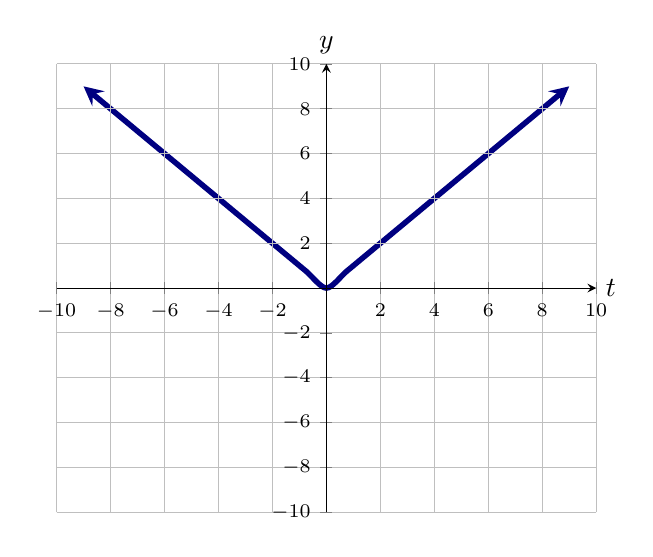
\begin{tikzpicture}
  \begin{axis}[
            domain=-10:10, ymax=10, xmax=10, ymin=-10, xmin=-10,
            axis lines =center, xlabel=$t$, ylabel=$y$, grid = major,
            ytick={-10,-8,-6,-4,-2,2,4,6,8,10},
            xtick={-10,-8,-6,-4,-2,2,4,6,8,10},
            ticklabel style={font=\scriptsize},
            every axis y label/.style={at=(current axis.above origin),anchor=south},
            every axis x label/.style={at=(current axis.right of origin),anchor=west},
            axis on top
          ]
          

          \addplot [line width=2, penColor, smooth, domain=(-9:9), <->] {abs(x)};
   


           

  \end{axis}
\end{tikzpicture}
\end{image}







\begin{example}

Solve $|m| = 18$.


Either $m = 18$  or $m = -18$

\end{example}




\subsection*{Continuity}


The absolute value function is a continuous function.

\begin{itemize}
\item On $(-\infty, 0)$ we have $| x | = -x$, which is a linear function, which is continuous.
\item On $[0, \infty)$ we have $| x | = x$, which is a linear function, which is continuous.
\end{itemize}


Both sides match up at $0$, since 

\[
\lim\limits_{x \to 0^-} |x| = 0
\]






That graph suggests that $|x|$ decreases on $(-\infty, 0]$  and  increases on $[0, \infty )$.  \\

This is confirmed by the formula. \\


On $(-\infty, 0]$, $|x| = -x$, which is a decreasing linear functions. \\


On $[0, \infty)$, $|x| = x$, which is an increasing linear functions. \\


\begin{example}  Behavior ($iRoC$)


Using the $iRoC$ to say where $A(x) = | x |$ increasing and decreasing. \\



\begin{explanation}


First, get rid of the absolute value bars.

\begin{itemize}
\item $x < 0$ when $|x| = \answer{-x}$
\item $x > 0$ when $|x| = \answer{x}$
\end{itemize}



\[
|x| = 
\begin{cases}
  -x & \text{ on } (-\infty, 0)   \\
  x  & \text{ on } [0, \infty)
\end{cases}
\]



Each piece is a restricted linear function.  We can get their $iRoC$.


\[
iRoC_{|x|} = 
\begin{cases}
  -1 & \text{ on } (-\infty, 0)   \\
  1  & \text{ on } (0, \infty).
\end{cases}
\]

$iRoC_{|x|}$ is negative on $(-\infty, 0)$ and positive on $(0, \infty)$. \\


$| x |$ is decreasing on $(-\infty, 0)$ and increasing on $(0, \infty)$.



\end{explanation}


\end{example}




Absolute value is a continuous function, which is decreasing on $(-\infty, 0)$ and increasing on $(0, \infty)$. That makes $| 0 | = 0$ the global minimum. \\


Since the absolute value function is a increasing linear function on $(0, \infty)$, we know that

\[
\lim\limits_{x \to \infty}| x | = \infty
\]



Therefore, the range is $[0, \infty)$.








\begin{example}  Critical Numbers


What are the cricital numbers for $A(x) = | x |$ ?



\begin{explanation}


First, $0$ is in the domain. \\

The previous examples shows that the $iRoC_{|x|}$ is defined and nonzero everywhere except $0$. \\

The only possible critical number is $0$.  We will show that there is no tangent line at $(0,0)$. \\


Suppose there is a tangent line to the graph of $y = | x |$ at $(0,0)$.  Then, it has to match the slope on the left, which is $-1$ and it has to match the slope on the right, which is $1$.  A line cannot have two slopes. \\ 


There is not tangent line at $(0,0)$, which means there is no slope. \\



\[
iRoC_{|x|}(0) \, \text{ does not exist }
\]


$0$ is the only critical number.



\end{explanation}


\end{example}








\begin{definition} \textbf{\textcolor{green!50!black}{Absolute Functions}}

Absolute functions are those functions that \textbf{\textcolor{purple!85!blue}{can}} be represented by formulas of the form


\[      AV(x) = A \cdot | B \, x + C| + D   \]

where $A$, $B$, $C$, and $D$ are real numbers, with $A \ne B$ and $B \ne 0$ is a nonzero real number.


\end{definition}


\textbf{Note:}  In the template for absolute value functions, There is a leading coefficient for the function and there is a leading coefficient for the linear function inside the absolute value bars. \\



\begin{example}  Behavior


Rewrite $A(x) = | x - 3|$ without absolute value bars.



\begin{explanation}


First, get rid of the absolute value bars.

\begin{itemize}
\item $x - 3 < 0$ when $x < \answer{3}$
\item $x - 3 > 0$ when $x > \answer{3}$
\end{itemize}



\[
A(x) = 
\begin{cases}
  -(x - 3) & \text{ on } (-\infty, 3)   \\
  x - 3  & \text{ on } [3, \infty).
\end{cases}
\]






\end{explanation}


\end{example}


















\begin{center}
\textbf{\textcolor{green!50!black}{ooooo-=-=-=-ooOoo-=-=-=-ooooo}} \\

more examples can be found by following this link\\ \link[More Examples of Elementary Functions]{https://ximera.osu.edu/csccmathematics/precalculus1/precalculus1/elementaryLibrary2/examples/exampleList}

\end{center}







\end{document}
